% =====================================================================
%  Người B -- Task 3: Thiết kế kiến trúc
%  Nguồn: docs/architecture/adr/*.md, docs/architecture/deployment-diagram.puml,
%         docs/deployment.md, docs/database-design.md
%  Ngân sách: ~3,5 trang
% =====================================================================
\section{Task 3 -- Thiết kế kiến trúc}

\subsection{Task 3.1 -- Phương pháp và quyết định kiến trúc}

% TODO(B): viết docs/architecture/architecture.md trước (1-2 trang), sau đó tóm tắt vào đây.
% Nội dung bắt buộc theo đề:
%   - kiến trúc phân lớp + C4 container;
%   - Next.js/PWA, NestJS module/domain, PostgreSQL + migration;
%   - dịch vụ thanh toán mô phỏng (ZaloPay Sandbox);
%   - logging, health check, quản lý cấu hình;
%   - lý do chọn, ưu điểm, hạn chế, trade-off.

\paragraph{Kiến trúc phân lớp.}
% TODO(B): 1 đoạn + bảng 9 module API và trách nhiệm (lấy từ as2.tex cũ mục 4).
\begin{table}[H]
\centering\small
\caption{Các module nghiệp vụ của API}
\label{tabB:modules}
\begin{tabularx}{\textwidth}{@{}l X@{}}
\toprule
\textbf{Module} & \textbf{Trách nhiệm} \\
\midrule
% TODO(B): auth, users, products, cart, orders, payments, ingredients, recipes, stock-imports
\bottomrule
\end{tabularx}
\end{table}

\paragraph{Logging, health check và cấu hình.}
% TODO(B): 3 đoạn ngắn: transform/exception interceptor + log request;
% GET /api/v1/health trả trạng thái API + DB; toàn bộ config qua env, .env.example, không commit secret.

\paragraph{Ưu điểm, hạn chế và trade-off.}
% TODO(B): bảng 3 cột: Quyết định | Ưu điểm | Hạn chế / trade-off.
\begin{table}[H]
\centering\small
\caption{Trade-off của các quyết định kiến trúc}
\label{tabB:tradeoff}
\begin{tabularx}{\textwidth}{@{}p{5cm} X X@{}}
\toprule
\textbf{Quyết định} & \textbf{Ưu điểm} & \textbf{Hạn chế / trade-off} \\
\midrule
% TODO(B): monorepo, modular monolith, Prisma, ZaloPay sandbox, deploy PaaS free tier
\bottomrule
\end{tabularx}
\end{table}

\subsection{Task 3.2 -- Hồ sơ quyết định kiến trúc (ADR)}
% TODO(B): tóm tắt 2 ADR có sẵn, mỗi cái 1 bảng ngắn: Bối cảnh | Quyết định | Hệ quả.
% Nguồn: docs/architecture/adr/001-monorepo.md, 002-payment-zalopay-sandbox.md.
% Ghi rõ đường dẫn để truy vết.
\begin{table}[H]
\centering\small
\caption{ADR 001 -- Monorepo}
\label{tabB:adr1}
\begin{tabularx}{\textwidth}{@{}p{3cm} X@{}}
\toprule
\textbf{Mục} & \textbf{Nội dung} \\
\midrule
% TODO(B): điền 3 dòng dưới
Bối cảnh & \\
Quyết định & \\
Hệ quả & \\
\bottomrule
\end{tabularx}
\end{table}

\begin{table}[H]
\centering\small
\caption{ADR 002 -- ZaloPay Sandbox thay cho mock payment}
\label{tabB:adr2}
\begin{tabularx}{\textwidth}{@{}p{3cm} X@{}}
\toprule
\textbf{Mục} & \textbf{Nội dung} \\
\midrule
% TODO(B): điền 3 dòng dưới
Bối cảnh & \\
Quyết định & \\
Hệ quả & \\
\bottomrule
\end{tabularx}
\end{table}

\subsection{Task 3.3 -- Deployment diagram}
% TODO(B): export deployment-diagram.puml -> .svg (đề yêu cầu cả nguồn và ảnh kết xuất).
% Sơ đồ phải thể hiện: thiết bị người dùng, Vercel/CDN, Render container, Neon + persistent
% storage, registry/nền tảng deploy, HTTPS + cổng nội bộ, secret/env, health check, log,
% ranh giới local - CI - production.
\begin{figure}[H]
\centering
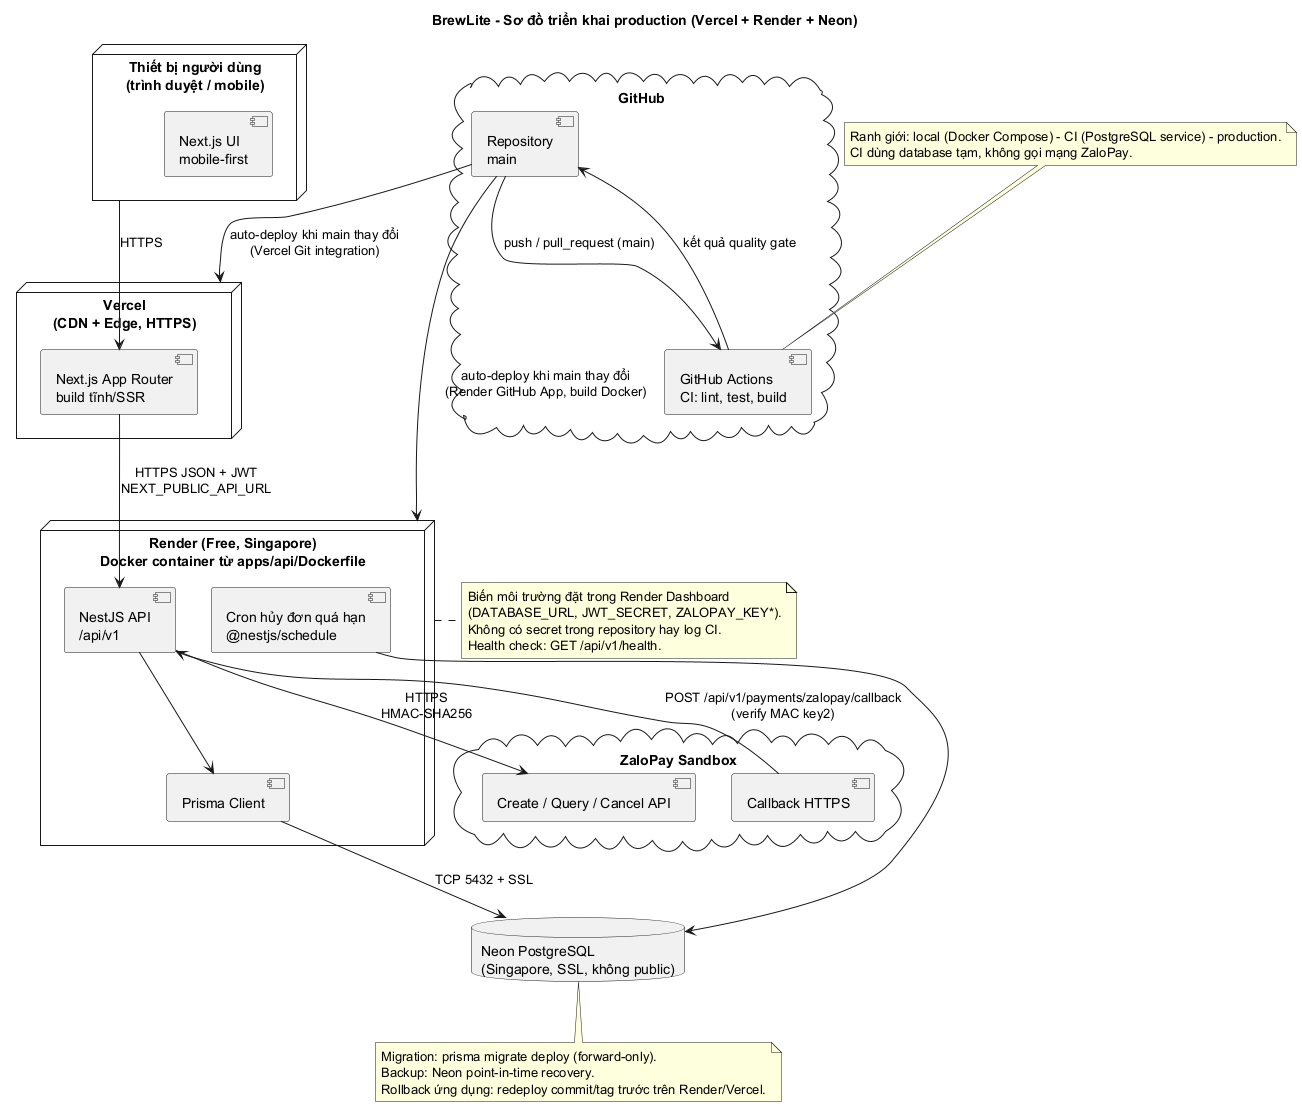
\includegraphics[width=0.78\textwidth]{../figures/diagrams/BrewLite-Deployment.png}
\caption{Deployment diagram production: Vercel -- Render -- Neon -- ZaloPay -- GitHub Actions}
\label{figB:deploy}
\end{figure}

\paragraph{Đối chiếu container với mã nguồn.}
% TODO(B): bảng: Container/dịch vụ | Thành phần kiến trúc | Bằng chứng trong repo.
% (tiêu chí nghiệm thu Task 3.2: truy vết được mỗi container tới code)
\begin{table}[H]
\centering\small
\caption{Truy vết container trong deployment diagram}
\label{tabB:deploy-trace}
\begin{tabularx}{\textwidth}{@{}l X X@{}}
\toprule
\textbf{Container} & \textbf{Thành phần} & \textbf{Bằng chứng} \\
\midrule
% TODO(B): Web, API, DB, Payment, CI
\bottomrule
\end{tabularx}
\end{table}
